Under the condition of \textbeta-stable, the proton's contribution $x_p = n_p/n_b$ to the baryon density of of neutrino-free \gls{NS} matter is given by Figure \ref{fig:xp}, computed with 5 different versions of the density-dependent \gls{NN} interaction. For simplicity, the baryon spin polarization $\Delta$ is assumed to be density-independent, such that it can be varied separatedly from $\Delta=0$ (spin saturated scenario) to $\Delta = 1$ (total polarization). It can be seen from Figure \ref{fig:xp} that in all cases, the higher the density, the more protons there are in the baryon composition. Furthermore, with the newly introduced parameterization of spin-dependent terms (10 and 11) in all 5 interactions, generally the protons are more abundant at higher polarization, the central density corresponding to the highest possible \gls{NS} in each interaction also tends to decrease to a comparable level for each model with such change in $\Delta$.
\begin{figure}[ht!]
        \centering
        \includegraphics[width=\textwidth]{fig/xp.eps}
        \caption{Proton fraction $x_p$ of \textbeta-stable \gls{NM} at different baryon density and spin polarization for CDM3Y$n$ interactions. The lower horizontal lines are the \gls{DU} threshold \eqref{eq:xDU} and the dot at the end of each line corresponds to the highest mass \gls{NS}'s central density of each model.}
        \label{fig:xp}
\end{figure} 
The density-dependent proton fraction $x_p$ is also an essential input for determining the cooling rate of the \gls{NS}, in which the dominant direct Urca (\gls{DU}) process of \gls{NS} cooling by $\nu$ emission \citep{lattimer2004physics}, i.e.
\begin{equation}
    n \longrightarrow p + e^- +\bar{\nu}_e \quad\text{and}\quad p \longrightarrow n + e^+ + \nu_e,
\end{equation}
can only take place if the proton fraction exceeds the threshold \citep{loan2011equation}
\begin{equation}
    x_{DU} = \frac{1}{ 1 + \left[ 1 + \left( \frac{n_e}{n_e + n_\mu} \right)^{1/3} \right]^3 }
    \label{eq:xDU}
\end{equation}
Note that the thresholds $x_{DU}$ determined in these calculations remain fairly unchanged in the whole range of baryon density, as well as when the polarization varies or at different models, which can be explained by the absence of interaction between leptons and baryons in the current study. The proton fraction $x_p$ in this case increases significantly as the value of $\Delta$ rises from $0\to 1$ and surpasses the \gls{DU} threshold at much lower density of $\gtrsim 3n_0$. Beside, the electron fraction infered by this result might also reach up to $\gtrsim 20\%$ at $\Delta$ approaching $1$, which is fairly compatible with the observed quantity $27\%$ from the blue kilonova ejecta following the GW170817 event \citep{abbott2017gw170817, evans2017swift} and can very possibly come from a magnetar as suggested by \cite{metzger2018magnetar}.\par
\begin{figure}[ht!]
        \centering
        \includegraphics[width=\textwidth]{fig/symmetric.eps}
        \caption{Symmetric energy $S$ and energy per nucleon of symmetric \gls{NM} at increasing polarization with 5 CDM3Y$n$ interaction models. The shaded areas are the empirical ranges obtained from the Bayesian study \citep{xie2019bayesian} of the \gls{NS} of radius $R_{1.4}$ at 68\% and 90\% confident level (\gls{CFL}) with the GW170817 event \citep{abbott2018gw170817}.}
        \label{fig:s}
\end{figure} 
On one hand, as shown in Figure \ref{fig:s}, the total energy density of the $npe\mu$ matter doesn't vary much from each others and from different configurations, while on the other hand, 
\begin{figure}[ht!]
        \centering
        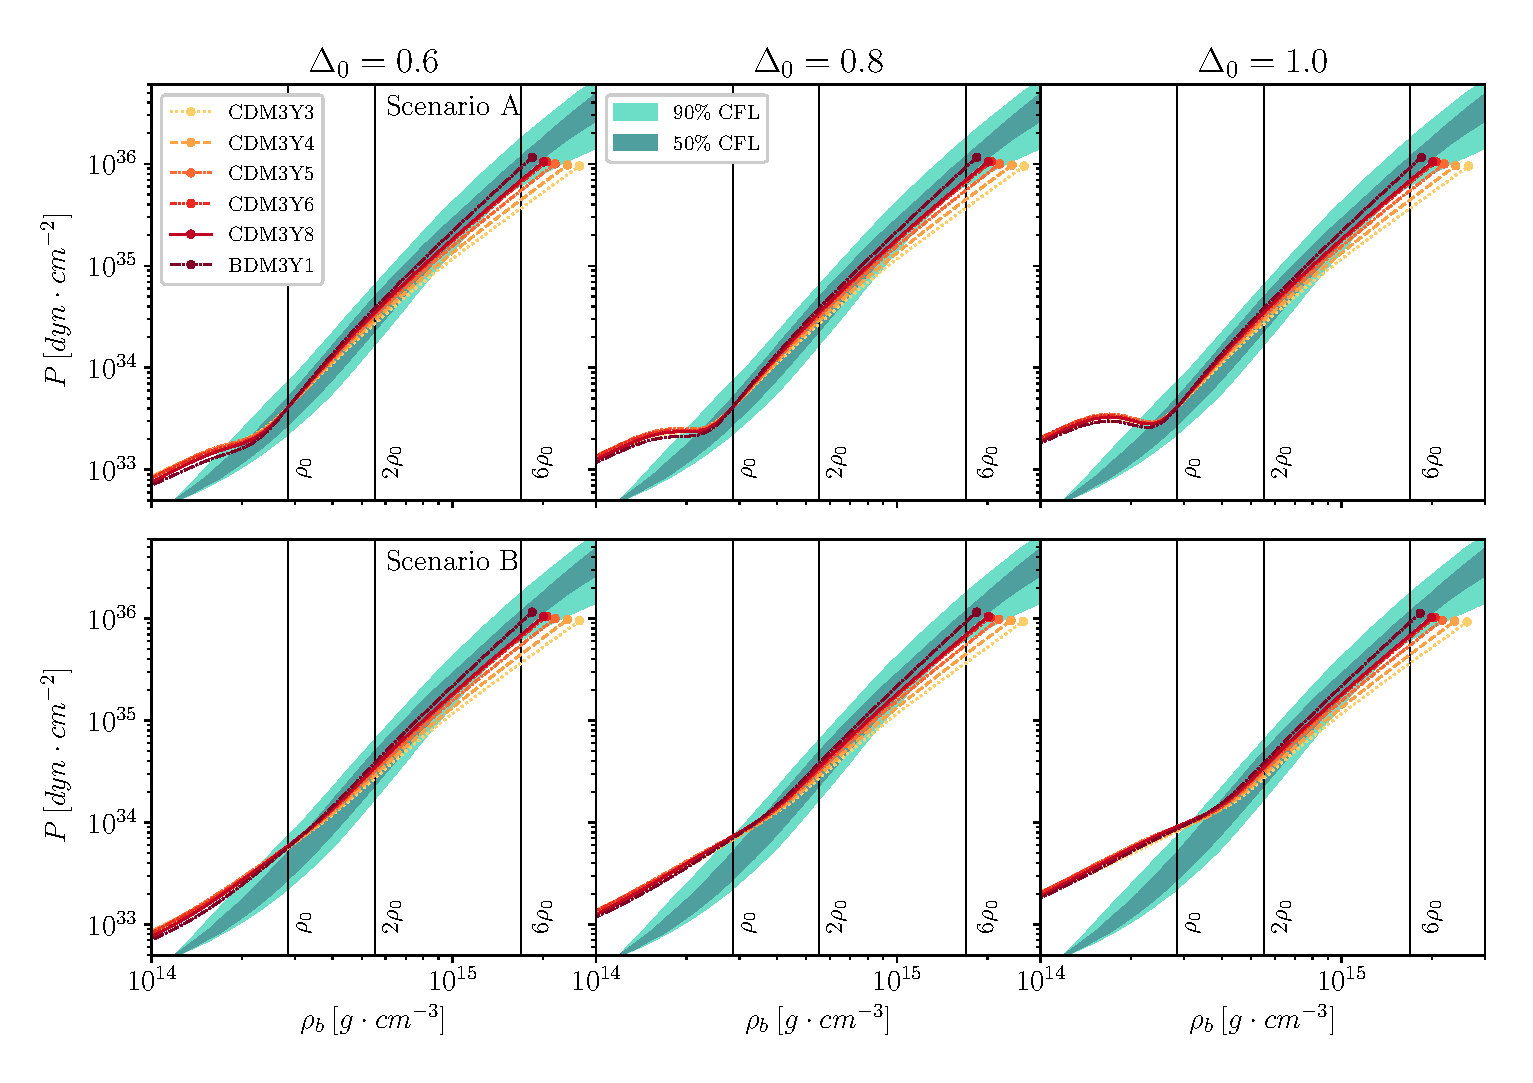
\includegraphics[width=\textwidth]{fig/P.eps}
        \caption{Same as Figure \ref{fig:s} for the pressure $P$ along with empirical pressure given by the ``Spectral'' \gls{EoS} from the Bayesian analysis of the GW170817 data \citep{abbott2018gw170817} with 50\% (light gray) and 90\% (dark gray) confidence level. The dot at the end of each line corresponds to the central baryon density $n_b$ of maximum \gls{NS} mass.}
        \label{fig:p}
\end{figure} 
\begin{figure}[ht!]
        \centering
        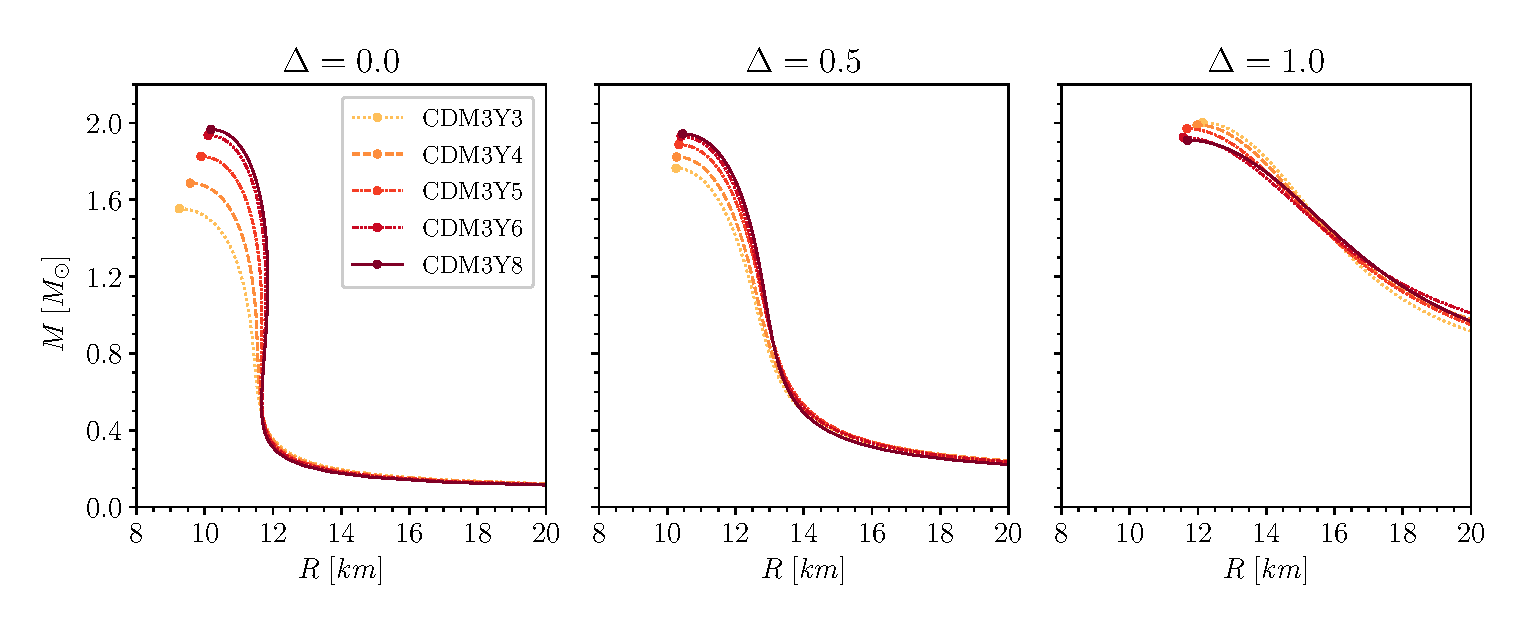
\includegraphics[width=\textwidth]{fig/MR.eps}
        \caption{The relation between gravitational mass $M$ and the radius $R$ of the \gls{NS} according to the corresponding model and polarization. The GW170817 constraint for \gls{NS} with mass $1.4M_\odot$ is shown by the colored contour, where the blue (red) shaded area represents the heavier (lighter) \gls{NS} \citep{abbott2018gw170817}. The dot in each line indicates the maximum \gls{NS} mass of the each model. The dark and light orange region indicates the mass of the second \gls{PSR} J0348+0432 \citep{antoniadis2013massive} and millisecond \gls{PSR} J0740+6620 \citep{cromartie2020relativistic} respectively, which are the heaviest \glsplural{NS} ever observed.}
        \label{fig:mr}
\end{figure} 
\begin{figure}[ht!]
        \centering
        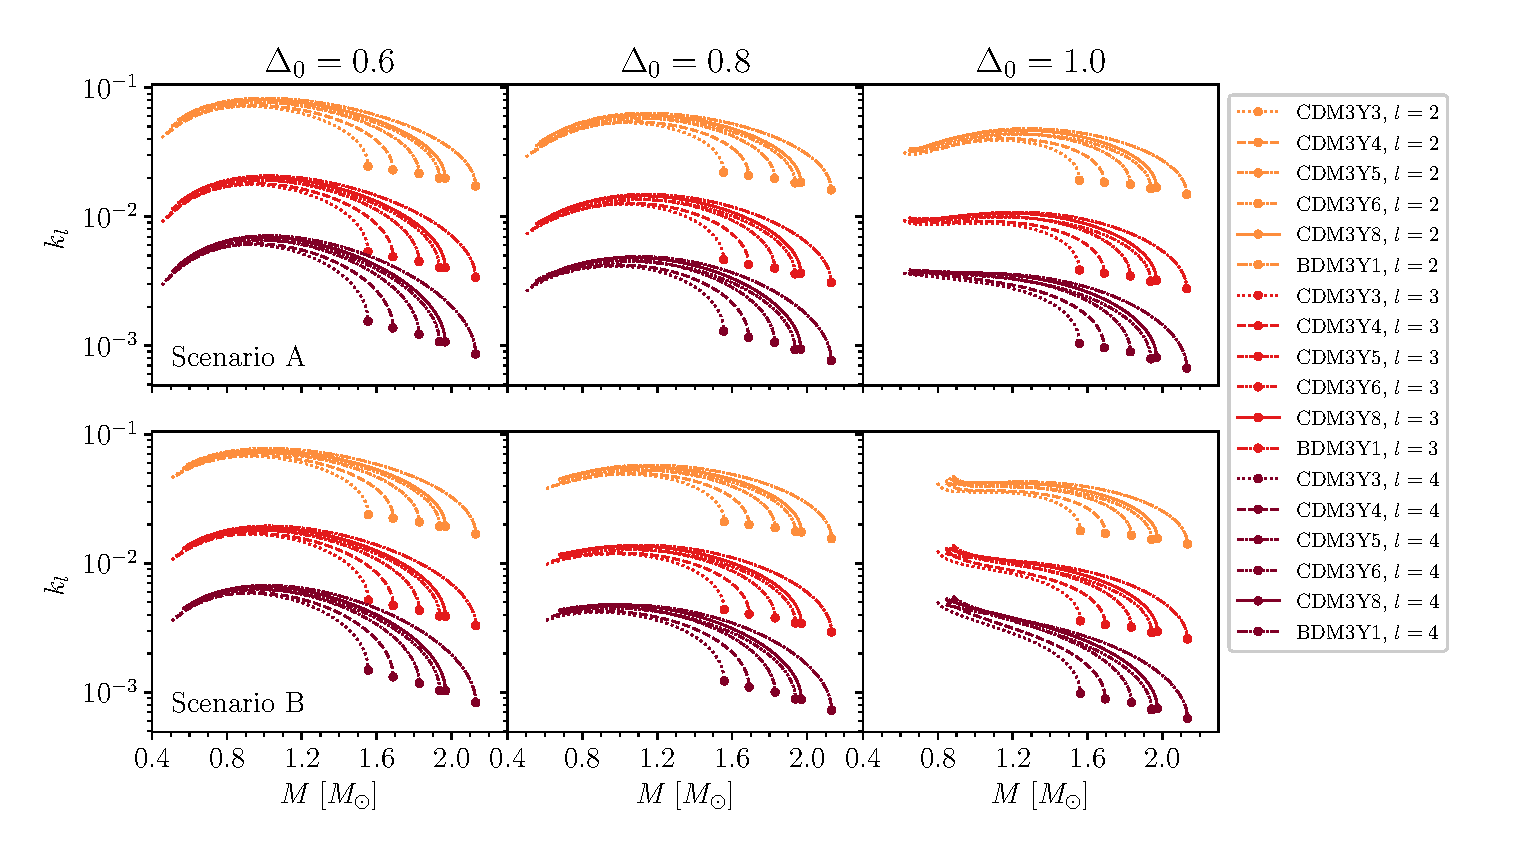
\includegraphics[width=\textwidth]{fig/kl.eps}
        \caption{\gls{GE} tidal Love number at $l$\textsuperscript{th} order $k_l$ as function of \gls{NS} mass computed with CDM3Y$n$ models at different spin polarizations.}
        \label{fig:kl}
\end{figure} 
\begin{figure}[ht!]
    \centering
    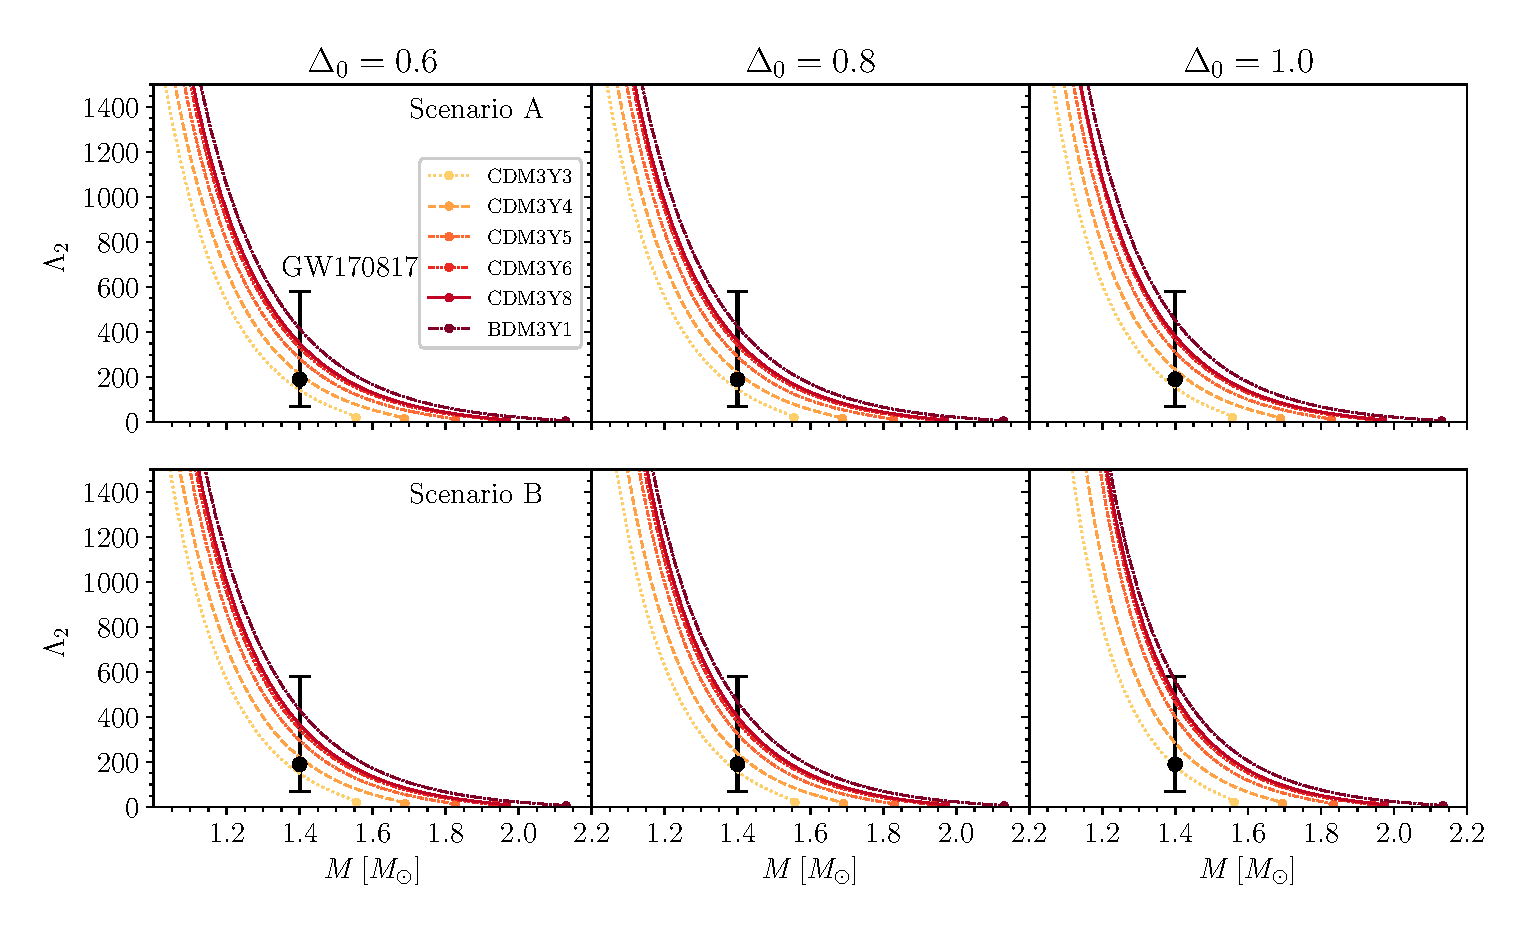
\includegraphics[width=\textwidth]{fig/Lambda2.eps}
    \caption{Dimensionless \gls{GE} tidal deformability parameter of 2\textsuperscript{nd} order $\Lambda_2$ of different CDM3Y$n$ models with varying $\Delta$. The vertical bar is the empirical tidal deformability constraint $\Lambda_2 \approx 190_{-120}^{+390}$ at $1.4M_\odot$, obtained from the Bayesian analysis of GW170817 data with 90\% confidence level \citep{abbott2018gw170817}.}
    \label{fig:Lambda2}
\end{figure} 
\begin{figure}[ht!]
        \centering
        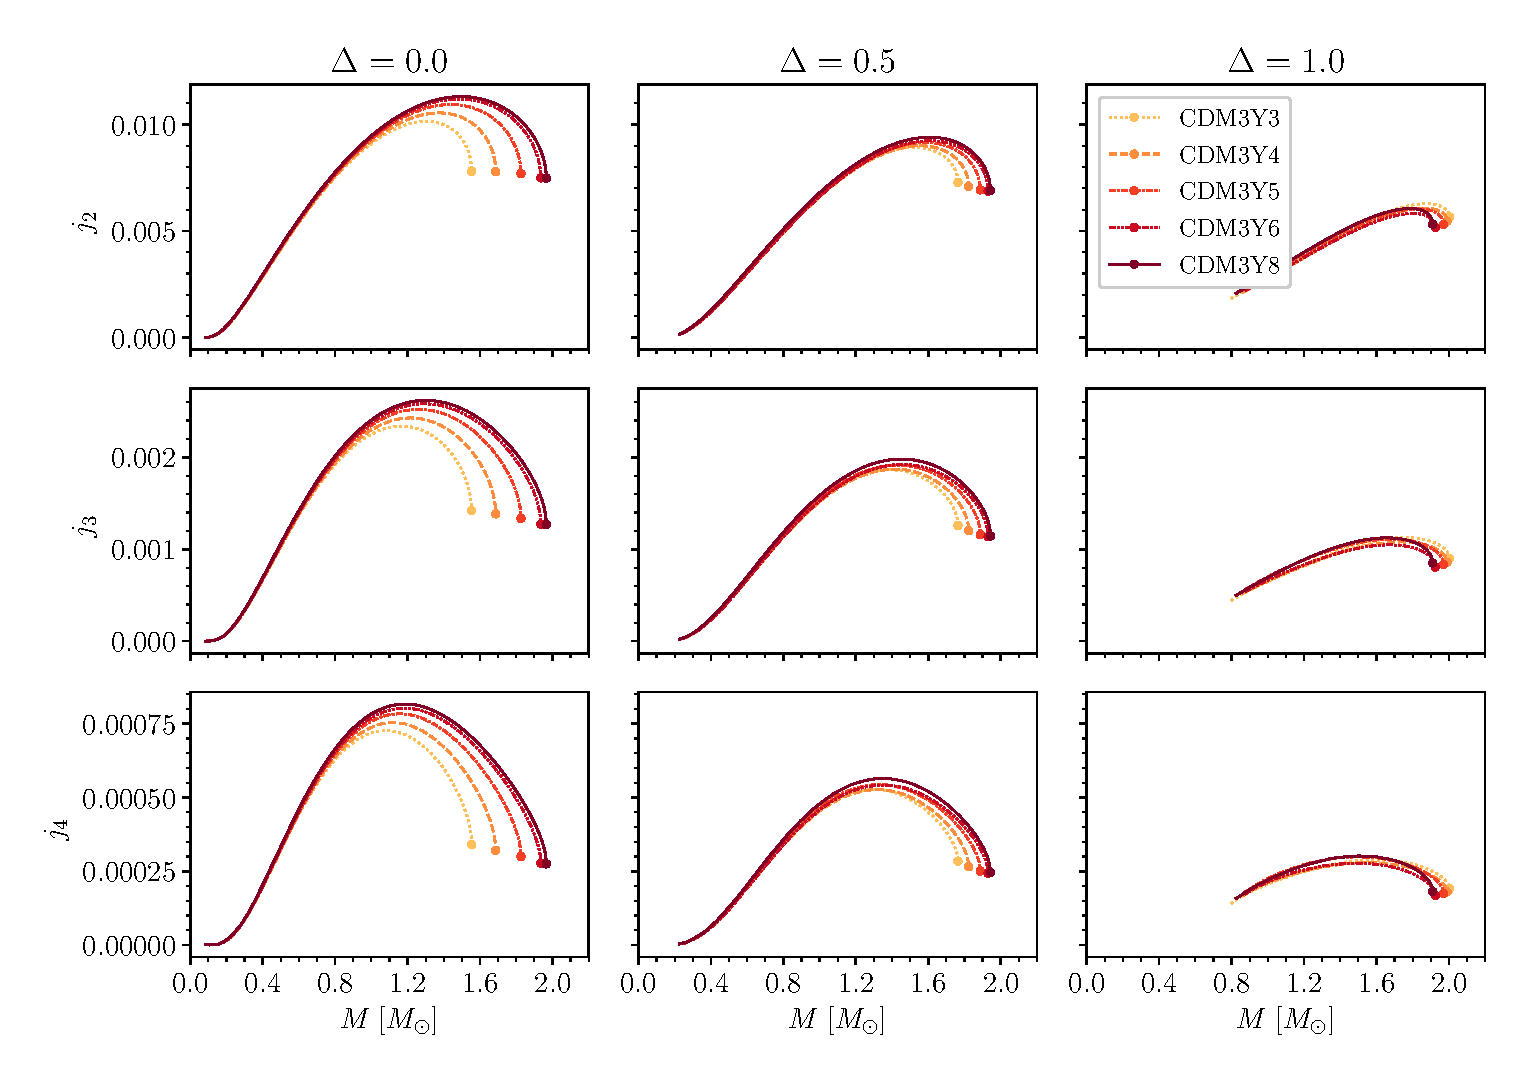
\includegraphics[width=\textwidth]{fig/jl_stat.eps}
        \caption{\gls{GM} tidal Love number at $l$\textsuperscript{nd} order $j_l$ as function of \gls{NS} mass computed with CDM3Y$n$ models of \emph{strictly static fluid} at different polarizations.}
        \label{fig:jl_stat}
\end{figure} 
\begin{figure}[ht!]
        \centering
        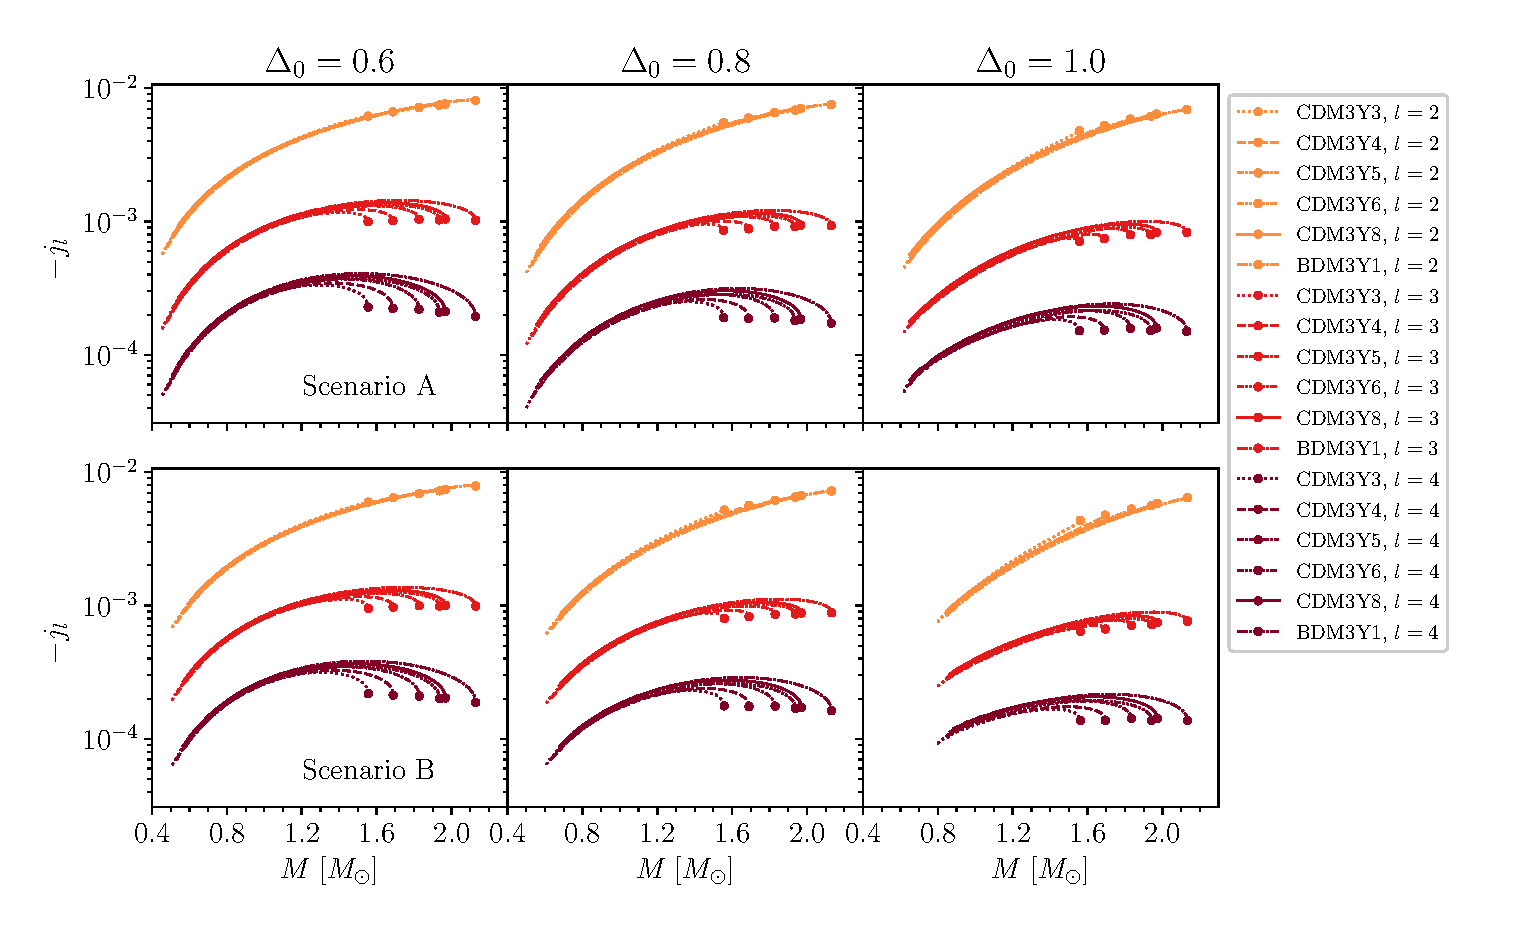
\includegraphics[width=\textwidth]{fig/jl_irrot.eps}
        \caption{\gls{GM} tidal Love number at $l$\textsuperscript{nd} order $j_l$ as function of \gls{NS} mass computed with CDM3Y$n$ models of \emph{irrotational fluid} at different polarizations.}
        \label{fig:jl_irrot}
\end{figure} 
